\documentclass[12pt,]{article}
\usepackage{lmodern}
\usepackage{amssymb,amsmath}
\usepackage{ifxetex,ifluatex}
\usepackage{fixltx2e} % provides \textsubscript
\ifnum 0\ifxetex 1\fi\ifluatex 1\fi=0 % if pdftex
  \usepackage[T1]{fontenc}
  \usepackage[utf8]{inputenc}
\else % if luatex or xelatex
  \ifxetex
    \usepackage{mathspec}
  \else
    \usepackage{fontspec}
  \fi
  \defaultfontfeatures{Ligatures=TeX,Scale=MatchLowercase}
\fi
% use upquote if available, for straight quotes in verbatim environments
\IfFileExists{upquote.sty}{\usepackage{upquote}}{}
% use microtype if available
\IfFileExists{microtype.sty}{%
\usepackage{microtype}
\UseMicrotypeSet[protrusion]{basicmath} % disable protrusion for tt fonts
}{}
\usepackage[margin=1in]{geometry}
\usepackage{hyperref}
\hypersetup{unicode=true,
            pdftitle={Yeast Genetic Interactions Network},
            pdfborder={0 0 0},
            breaklinks=true}
\urlstyle{same}  % don't use monospace font for urls
\usepackage{color}
\usepackage{fancyvrb}
\newcommand{\VerbBar}{|}
\newcommand{\VERB}{\Verb[commandchars=\\\{\}]}
\DefineVerbatimEnvironment{Highlighting}{Verbatim}{commandchars=\\\{\}}
% Add ',fontsize=\small' for more characters per line
\usepackage{framed}
\definecolor{shadecolor}{RGB}{248,248,248}
\newenvironment{Shaded}{\begin{snugshade}}{\end{snugshade}}
\newcommand{\KeywordTok}[1]{\textcolor[rgb]{0.13,0.29,0.53}{\textbf{{#1}}}}
\newcommand{\DataTypeTok}[1]{\textcolor[rgb]{0.13,0.29,0.53}{{#1}}}
\newcommand{\DecValTok}[1]{\textcolor[rgb]{0.00,0.00,0.81}{{#1}}}
\newcommand{\BaseNTok}[1]{\textcolor[rgb]{0.00,0.00,0.81}{{#1}}}
\newcommand{\FloatTok}[1]{\textcolor[rgb]{0.00,0.00,0.81}{{#1}}}
\newcommand{\ConstantTok}[1]{\textcolor[rgb]{0.00,0.00,0.00}{{#1}}}
\newcommand{\CharTok}[1]{\textcolor[rgb]{0.31,0.60,0.02}{{#1}}}
\newcommand{\SpecialCharTok}[1]{\textcolor[rgb]{0.00,0.00,0.00}{{#1}}}
\newcommand{\StringTok}[1]{\textcolor[rgb]{0.31,0.60,0.02}{{#1}}}
\newcommand{\VerbatimStringTok}[1]{\textcolor[rgb]{0.31,0.60,0.02}{{#1}}}
\newcommand{\SpecialStringTok}[1]{\textcolor[rgb]{0.31,0.60,0.02}{{#1}}}
\newcommand{\ImportTok}[1]{{#1}}
\newcommand{\CommentTok}[1]{\textcolor[rgb]{0.56,0.35,0.01}{\textit{{#1}}}}
\newcommand{\DocumentationTok}[1]{\textcolor[rgb]{0.56,0.35,0.01}{\textbf{\textit{{#1}}}}}
\newcommand{\AnnotationTok}[1]{\textcolor[rgb]{0.56,0.35,0.01}{\textbf{\textit{{#1}}}}}
\newcommand{\CommentVarTok}[1]{\textcolor[rgb]{0.56,0.35,0.01}{\textbf{\textit{{#1}}}}}
\newcommand{\OtherTok}[1]{\textcolor[rgb]{0.56,0.35,0.01}{{#1}}}
\newcommand{\FunctionTok}[1]{\textcolor[rgb]{0.00,0.00,0.00}{{#1}}}
\newcommand{\VariableTok}[1]{\textcolor[rgb]{0.00,0.00,0.00}{{#1}}}
\newcommand{\ControlFlowTok}[1]{\textcolor[rgb]{0.13,0.29,0.53}{\textbf{{#1}}}}
\newcommand{\OperatorTok}[1]{\textcolor[rgb]{0.81,0.36,0.00}{\textbf{{#1}}}}
\newcommand{\BuiltInTok}[1]{{#1}}
\newcommand{\ExtensionTok}[1]{{#1}}
\newcommand{\PreprocessorTok}[1]{\textcolor[rgb]{0.56,0.35,0.01}{\textit{{#1}}}}
\newcommand{\AttributeTok}[1]{\textcolor[rgb]{0.77,0.63,0.00}{{#1}}}
\newcommand{\RegionMarkerTok}[1]{{#1}}
\newcommand{\InformationTok}[1]{\textcolor[rgb]{0.56,0.35,0.01}{\textbf{\textit{{#1}}}}}
\newcommand{\WarningTok}[1]{\textcolor[rgb]{0.56,0.35,0.01}{\textbf{\textit{{#1}}}}}
\newcommand{\AlertTok}[1]{\textcolor[rgb]{0.94,0.16,0.16}{{#1}}}
\newcommand{\ErrorTok}[1]{\textcolor[rgb]{0.64,0.00,0.00}{\textbf{{#1}}}}
\newcommand{\NormalTok}[1]{{#1}}
\usepackage{longtable,booktabs}
\usepackage{graphicx,grffile}
\makeatletter
\def\maxwidth{\ifdim\Gin@nat@width>\linewidth\linewidth\else\Gin@nat@width\fi}
\def\maxheight{\ifdim\Gin@nat@height>\textheight\textheight\else\Gin@nat@height\fi}
\makeatother
% Scale images if necessary, so that they will not overflow the page
% margins by default, and it is still possible to overwrite the defaults
% using explicit options in \includegraphics[width, height, ...]{}
\setkeys{Gin}{width=\maxwidth,height=\maxheight,keepaspectratio}
\IfFileExists{parskip.sty}{%
\usepackage{parskip}
}{% else
\setlength{\parindent}{0pt}
\setlength{\parskip}{6pt plus 2pt minus 1pt}
}
\setlength{\emergencystretch}{3em}  % prevent overfull lines
\providecommand{\tightlist}{%
  \setlength{\itemsep}{0pt}\setlength{\parskip}{0pt}}
\setcounter{secnumdepth}{5}
% Redefines (sub)paragraphs to behave more like sections
\ifx\paragraph\undefined\else
\let\oldparagraph\paragraph
\renewcommand{\paragraph}[1]{\oldparagraph{#1}\mbox{}}
\fi
\ifx\subparagraph\undefined\else
\let\oldsubparagraph\subparagraph
\renewcommand{\subparagraph}[1]{\oldsubparagraph{#1}\mbox{}}
\fi

%%% Use protect on footnotes to avoid problems with footnotes in titles
\let\rmarkdownfootnote\footnote%
\def\footnote{\protect\rmarkdownfootnote}

%%% Change title format to be more compact
\usepackage{titling}

% Create subtitle command for use in maketitle
\newcommand{\subtitle}[1]{
  \posttitle{
    \begin{center}\large#1\end{center}
    }
}

\setlength{\droptitle}{-2em}
  \title{Yeast Genetic Interactions Network}
  \pretitle{\vspace{\droptitle}\centering\huge}
  \posttitle{\par}
  \author{}
  \preauthor{}\postauthor{}
  \date{}
  \predate{}\postdate{}


\begin{document}
\maketitle

{
\setcounter{tocdepth}{2}
\tableofcontents
}
\section{Genetic Interactions}\label{genetic-interactions}

A genetic interaction (GI) between two genes generally indicates that
the phenotype of a double mutant differs from what is expected from each
individual mutant. The existence of a GI between two genes does not
necessarily imply that these two genes code for interacting proteins or
that the two genes are even expressed in the same cell. In fact, a GI
only implies that the two genes share a functional relationship. These
two genes may be involved in the same biological process or pathway; or
they may also be involved in compensatory pathways with unrelated
apparent function {[}Genetic interaction networks: better understand to
better predict{]}

\section{Data}\label{data}

Here we will explore and analyse the GI network of yeast. Data were
downloaded from \href{https://thebiogrid.org/download.php}{BIOGRID} in
December 2016 and were sorted by organism under the hyperlink:
\textbf{BIOGRID-ORGANISM-3.4.143.tab2.zip}. We will use data from
\emph{Saccharomyces cerevisiae}. Files are in Tab2 format, so in order
to import them in r, we first have to remove manually the text from the
first part of the file.

The file from yeast contains many interactions. From them we have to
retrieve the ones we are interested in, which are the ones resulting
from
\href{https://en.wikipedia.org/wiki/Synthetic_genetic_array}{Synthetic
Genetic Arrays}.

\begin{Shaded}
\begin{Highlighting}[]
\KeywordTok{summary}\NormalTok{(yeast_BIOGRID$EXPERIMENTAL_SYSTEM)}
\end{Highlighting}
\end{Shaded}

\begin{verbatim}
## Affinity Capture-Luminescence           Affinity Capture-MS 
##                            50                         58455 
##          Affinity Capture-RNA      Affinity Capture-Western 
##                         11166                         16569 
##          Biochemical Activity          Co-crystal Structure 
##                          6650                           881 
##              Co-fractionation               Co-localization 
##                           975                           675 
##               Co-purification          Dosage Growth Defect 
##                          4326                          1988 
##              Dosage Lethality                 Dosage Rescue 
##                          1627                          5663 
##                   Far Western                          FRET 
##                           101                           219 
##              Negative Genetic                           PCA 
##                        115467                          6577 
##        Phenotypic Enhancement        Phenotypic Suppression 
##                          7487                          6590 
##              Positive Genetic               Protein-peptide 
##                         24681                           846 
##                   Protein-RNA         Reconstituted Complex 
##                           573                          7657 
##       Synthetic Growth Defect  Synthetic Haploinsufficiency 
##                         25200                           283 
##           Synthetic Lethality              Synthetic Rescue 
##                         16217                          6905 
##                    Two-hybrid 
##                         15973
\end{verbatim}

These are

\begin{itemize}
\tightlist
\item
  Negative: \textbf{Synthetic Lethality} and \textbf{Negative Genetic}
\item
  Positive: \textbf{Synthetic Rescue} and \textbf{Positive Genetic}
\end{itemize}

\subsection{Extract GIN}\label{extract-gin}

These four types of genetic relations are defined based on their
differentietion from un expected phenotype. The expected phenotype is

\textbf{Synthetic Lethality} means that the second mutation is lethal.
\textbf{Negative Genetic} means that the phenotype of the two mutations
is worse than expected. \textbf{Synthetic Rescue} means that even though
the first mutation is leathal, the second mutation regains the viability
of the organism. \textbf{Positive Genetic} means that the phenotype is
better (highest fitness) than expected.

\begin{Shaded}
\begin{Highlighting}[]
\NormalTok{yeast_GIN <-}\StringTok{ }\KeywordTok{subset}\NormalTok{(}\DataTypeTok{x =} \NormalTok{yeast_BIOGRID, EXPERIMENTAL_SYSTEM==}\StringTok{"Synthetic Lethality"} \NormalTok{|}\StringTok{ }\NormalTok{EXPERIMENTAL_SYSTEM==}\StringTok{"Negative Genetic"} \NormalTok{|}\StringTok{ }\NormalTok{EXPERIMENTAL_SYSTEM==}\StringTok{"Synthetic Rescue"} \NormalTok{|}\StringTok{ }\NormalTok{EXPERIMENTAL_SYSTEM==}\StringTok{"Positive Genetic"}\NormalTok{)}
\NormalTok{yeast_GIN$weights <-}\StringTok{ }\KeywordTok{with}\NormalTok{(yeast_GIN, }\KeywordTok{ifelse}\NormalTok{(EXPERIMENTAL_SYSTEM==}\StringTok{"Synthetic Lethality"} \NormalTok{|}\StringTok{ }\NormalTok{EXPERIMENTAL_SYSTEM==}\StringTok{"Negative Genetic"}\NormalTok{, -}\DecValTok{1}\NormalTok{, }\DecValTok{1}\NormalTok{))}

\KeywordTok{rm}\NormalTok{(yeast_BIOGRID)}

\KeywordTok{summary}\NormalTok{(yeast_GIN$EXPERIMENTAL_SYSTEM)}
\end{Highlighting}
\end{Shaded}

\begin{verbatim}
## Affinity Capture-Luminescence           Affinity Capture-MS 
##                             0                             0 
##          Affinity Capture-RNA      Affinity Capture-Western 
##                             0                             0 
##          Biochemical Activity          Co-crystal Structure 
##                             0                             0 
##              Co-fractionation               Co-localization 
##                             0                             0 
##               Co-purification          Dosage Growth Defect 
##                             0                             0 
##              Dosage Lethality                 Dosage Rescue 
##                             0                             0 
##                   Far Western                          FRET 
##                             0                             0 
##              Negative Genetic                           PCA 
##                        115467                             0 
##        Phenotypic Enhancement        Phenotypic Suppression 
##                             0                             0 
##              Positive Genetic               Protein-peptide 
##                         24681                             0 
##                   Protein-RNA         Reconstituted Complex 
##                             0                             0 
##       Synthetic Growth Defect  Synthetic Haploinsufficiency 
##                             0                             0 
##           Synthetic Lethality              Synthetic Rescue 
##                         16217                          6905 
##                    Two-hybrid 
##                             0
\end{verbatim}

The bar plot of the 4 types of relations.

\begin{Shaded}
\begin{Highlighting}[]
\KeywordTok{ggplot}\NormalTok{()+}
\StringTok{  }\KeywordTok{geom_bar}\NormalTok{(}\DataTypeTok{data =} \NormalTok{yeast_GIN, }\KeywordTok{aes}\NormalTok{(EXPERIMENTAL_SYSTEM, }\DataTypeTok{y=} \NormalTok{..count.., }\DataTypeTok{fill=}\NormalTok{EXPERIMENTAL_SYSTEM),}\DataTypeTok{show.legend =} \NormalTok{F)+}
\StringTok{  }\KeywordTok{ggtitle}\NormalTok{(}\StringTok{"Different Genetic Interactions in Yeast"}\NormalTok{)+}
\StringTok{  }\KeywordTok{labs}\NormalTok{(}\DataTypeTok{x=}\StringTok{"EXPERIMENTAL SYSTEM"}\NormalTok{, }\DataTypeTok{y=} \StringTok{"Number of genetic links"}\NormalTok{)+}
\StringTok{  }\KeywordTok{theme}\NormalTok{(}\DataTypeTok{panel.grid.major =} \KeywordTok{element_line}\NormalTok{(}\DataTypeTok{colour =} \StringTok{"grey90"}\NormalTok{), }\DataTypeTok{panel.background =} \KeywordTok{element_rect}\NormalTok{(}\DataTypeTok{fill =} \StringTok{"white"}\NormalTok{, }\DataTypeTok{colour =} \StringTok{"grey60"}\NormalTok{),}
        \DataTypeTok{axis.text.x =} \KeywordTok{element_text}\NormalTok{(}\DataTypeTok{size  =} \DecValTok{10}\NormalTok{, }\DataTypeTok{angle =} \DecValTok{45}\NormalTok{,}\DataTypeTok{hjust =} \DecValTok{1}\NormalTok{,}\DataTypeTok{vjust =} \DecValTok{1}\NormalTok{))}
\end{Highlighting}
\end{Shaded}

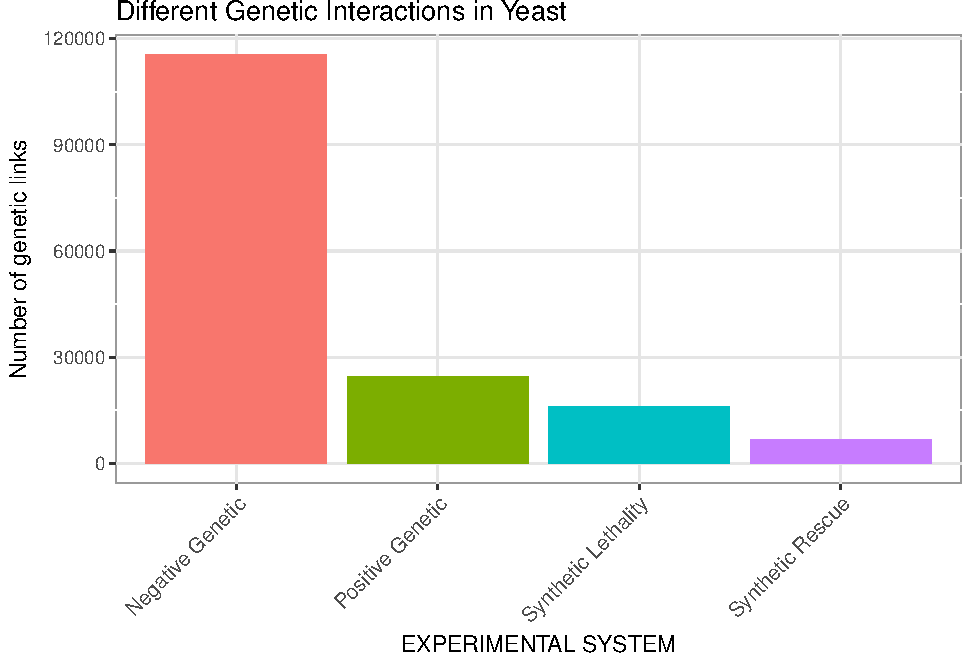
\includegraphics{yeast_GIN_files/figure-latex/unnamed-chunk-4-1.pdf}

\subsection{Duplicates and sign
consistency}\label{duplicates-and-sign-consistency}

We check for the unique links.In order to check this we first
concatenate the node IDs for each link and then we check for uniqueness.

\begin{Shaded}
\begin{Highlighting}[]
\NormalTok{yeast_GIN$links <-}\StringTok{ }\KeywordTok{with}\NormalTok{(yeast_GIN,}\KeywordTok{paste}\NormalTok{(yeast_GIN$INTERACTOR_A,yeast_GIN$INTERACTOR_B,}\DataTypeTok{sep =} \StringTok{","}\NormalTok{)) }\CommentTok{# concarnate in order to find duplicated links}
\KeywordTok{length}\NormalTok{(}\KeywordTok{unique}\NormalTok{(yeast_GIN$links)) }\CommentTok{# how many unique links}
\end{Highlighting}
\end{Shaded}

\begin{verbatim}
## [1] 144166
\end{verbatim}

But the number of links is:

\begin{Shaded}
\begin{Highlighting}[]
\KeywordTok{nrow}\NormalTok{(yeast_GIN)}
\end{Highlighting}
\end{Shaded}

\begin{verbatim}
## [1] 163270
\end{verbatim}

So there are 19104 duplicates. Next we want to label each link to see if
it's duplicated and after that we count the duplicates of each link in
order to find the origin of the duplicates.

\begin{Shaded}
\begin{Highlighting}[]
\NormalTok{yeast_GIN$duplicate <-}\StringTok{ }\KeywordTok{duplicated}\NormalTok{(yeast_GIN$links) |}\StringTok{ }\KeywordTok{duplicated}\NormalTok{(yeast_GIN$links, }\DataTypeTok{fromLast =} \OtherTok{TRUE}\NormalTok{) }\CommentTok{# returns TRUE for all duplicates, not the first ones only}

\NormalTok{yeast_GIN_dublicates <-}\StringTok{ }\KeywordTok{subset}\NormalTok{(}\DataTypeTok{x =} \NormalTok{yeast_GIN, yeast_GIN$duplicate==}\OtherTok{TRUE}\NormalTok{)}
\CommentTok{# count the number of occurences of each link}
\NormalTok{GIN_occurences <-}\StringTok{ }\NormalTok{yeast_GIN %>%}
\StringTok{  }\KeywordTok{group_by}\NormalTok{(links) %>%}
\StringTok{  }\KeywordTok{summarise} \NormalTok{(}\DataTypeTok{n =} \KeywordTok{n}\NormalTok{())}

\CommentTok{#summary(GIN_occurences)}
\end{Highlighting}
\end{Shaded}

\begin{Shaded}
\begin{Highlighting}[]
\NormalTok{GIN_occurences$link <-}\StringTok{ }\KeywordTok{c}\NormalTok{(}\KeywordTok{seq}\NormalTok{(}\DecValTok{1}\NormalTok{:}\KeywordTok{length}\NormalTok{(GIN_occurences$links)))}
\NormalTok{GIN_dupl_freq<-}\KeywordTok{aggregate}\NormalTok{(}\KeywordTok{rep.int}\NormalTok{(}\DecValTok{1}\NormalTok{, }\KeywordTok{length}\NormalTok{(GIN_occurences$link))~GIN_occurences$n, }\DataTypeTok{FUN=}\NormalTok{sum)}
\KeywordTok{names}\NormalTok{(GIN_dupl_freq)<-}\KeywordTok{c}\NormalTok{(}\StringTok{"Copies per link"}\NormalTok{,}\StringTok{"Count of links"}\NormalTok{)}
\KeywordTok{kable}\NormalTok{(GIN_dupl_freq, }\DataTypeTok{align =} \StringTok{'c'}\NormalTok{, }\DataTypeTok{caption =} \StringTok{"The number of copies of each link in the data yeast GIN"}\NormalTok{)}
\end{Highlighting}
\end{Shaded}

\begin{longtable}[]{@{}cc@{}}
\caption{The number of copies of each link in the data yeast
GIN}\tabularnewline
\toprule
Copies per link & Count of links\tabularnewline
\midrule
\endfirsthead
\toprule
Copies per link & Count of links\tabularnewline
\midrule
\endhead
1 & 129604\tabularnewline
2 & 11381\tabularnewline
3 & 2331\tabularnewline
4 & 593\tabularnewline
5 & 148\tabularnewline
6 & 55\tabularnewline
7 & 25\tabularnewline
8 & 8\tabularnewline
9 & 8\tabularnewline
10 & 2\tabularnewline
11 & 5\tabularnewline
12 & 2\tabularnewline
13 & 1\tabularnewline
14 & 1\tabularnewline
16 & 2\tabularnewline
\bottomrule
\end{longtable}

So some links appear multiple times. The link between YCR066W and
YJL092W appears 16 times in the dataset. This is due to the different
sources which discoved an already known genetic relation. Next we have
to delete duplicates. In order to do so we have to examine the nature of
the genetic interaction for each duplicate. If between duplicates there
are contradictions of the sign of the genetic interaction we have to
delete the interaction. If not, we'll keep one version of the
interaction.

\begin{Shaded}
\begin{Highlighting}[]
\NormalTok{## duplicated links}

\CommentTok{#sort links so the duplicates are adjacent? }
\NormalTok{duplicated_interactions <-}\StringTok{ }\NormalTok{yeast_GIN_dublicates[}\KeywordTok{order}\NormalTok{(yeast_GIN_dublicates$links),]}
\CommentTok{#yeast_GIN2 <- head(duplicated_interactions,n = 200)}
\NormalTok{yeast_GIN_unique_dup <-}\StringTok{ }\KeywordTok{as.data.frame}\NormalTok{(}\KeywordTok{matrix}\NormalTok{())}
\NormalTok{yeast_GIN_unique_dup <-}\StringTok{ }\KeywordTok{as.data.frame}\NormalTok{(}\KeywordTok{unique}\NormalTok{(duplicated_interactions$links))}
\NormalTok{yeast_GIN_unique_dup2 <-}\StringTok{ }\KeywordTok{as.data.frame}\NormalTok{(yeast_GIN_unique_dup)}

\NormalTok{ptm <-}\StringTok{ }\KeywordTok{proc.time}\NormalTok{()}
\NormalTok{for(i in }\DecValTok{1}\NormalTok{:}\KeywordTok{nrow}\NormalTok{(yeast_GIN_unique_dup))\{}

  \NormalTok{tmp_dupl_links <-}\StringTok{ }\KeywordTok{subset}\NormalTok{(yeast_GIN_dublicates,yeast_GIN_dublicates$links==yeast_GIN_unique_dup[i,])}
  
  \NormalTok{if (}\KeywordTok{abs}\NormalTok{(}\KeywordTok{sum}\NormalTok{(tmp_dupl_links$weights))==}\KeywordTok{nrow}\NormalTok{(tmp_dupl_links))\{}
    
    \NormalTok{yeast_GIN_unique_dup2[i,}\DecValTok{2}\NormalTok{] <-}\StringTok{ "consistent"}
    \CommentTok{#print(paste0("consistent ",yeast_GIN_unique_dup[i,1]))}
      
    \NormalTok{\} else \{}
      \NormalTok{yeast_GIN_unique_dup2[i,}\DecValTok{2}\NormalTok{] <-}\StringTok{ "inconsistent"}
      \CommentTok{#print(paste("inconsistent ",yeast_GIN_unique_dup[i,1]))}
    \NormalTok{\}}
 
  \NormalTok{yeast_GIN_unique_dup2[i,}\DecValTok{3}\NormalTok{] <-}\StringTok{ }\KeywordTok{length}\NormalTok{(}\KeywordTok{which}\NormalTok{(tmp_dupl_links$weights>}\DecValTok{0}\NormalTok{))}\CommentTok{#Positive_Interactions}
  \NormalTok{yeast_GIN_unique_dup2[i,}\DecValTok{4}\NormalTok{] <-}\StringTok{ }\KeywordTok{length}\NormalTok{(}\KeywordTok{which}\NormalTok{(tmp_dupl_links$weights<}\DecValTok{0}\NormalTok{)) }\CommentTok{#Positive_Interactions}
  \NormalTok{tmp_dupl_links <-}\StringTok{ }\KeywordTok{c}\NormalTok{()}
  
\NormalTok{\}}

\KeywordTok{colnames}\NormalTok{(yeast_GIN_unique_dup2) <-}\StringTok{ }\KeywordTok{c}\NormalTok{(}\StringTok{"Dublicated_Interactions"}\NormalTok{,}\StringTok{"Consistency"}\NormalTok{,}\StringTok{"Positive_Interactions"}\NormalTok{, }\StringTok{"Negative_Interactions"}\NormalTok{)}
\KeywordTok{proc.time}\NormalTok{() -}\StringTok{ }\NormalTok{ptm}
\end{Highlighting}
\end{Shaded}

\begin{verbatim}
##    user  system elapsed 
##  43.073   7.770  52.446
\end{verbatim}

\begin{Shaded}
\begin{Highlighting}[]
\CommentTok{#consistency}
\KeywordTok{ggplot}\NormalTok{()+}
\StringTok{  }\KeywordTok{geom_bar}\NormalTok{(}\DataTypeTok{data =} \NormalTok{yeast_GIN_unique_dup2, }\KeywordTok{aes}\NormalTok{(Consistency, }\DataTypeTok{y=} \NormalTok{..count.., }\DataTypeTok{fill=}\NormalTok{Consistency),}\DataTypeTok{show.legend =} \NormalTok{F)+}
\StringTok{  }\KeywordTok{ggtitle}\NormalTok{(}\StringTok{"Sign Consistency across duplicate genetic yeast interactions from BIOGRID"}\NormalTok{)+}
\StringTok{  }\KeywordTok{labs}\NormalTok{(}\DataTypeTok{x=}\StringTok{"Consistency"}\NormalTok{, }\DataTypeTok{y=} \StringTok{"Number of duplicate genetic links"}\NormalTok{)+}
\StringTok{  }\KeywordTok{theme}\NormalTok{(}\DataTypeTok{panel.grid.major =} \KeywordTok{element_line}\NormalTok{(}\DataTypeTok{colour =} \StringTok{"grey90"}\NormalTok{), }\DataTypeTok{panel.background =} \KeywordTok{element_rect}\NormalTok{(}\DataTypeTok{fill =} \StringTok{"white"}\NormalTok{, }\DataTypeTok{colour =} \StringTok{"grey60"}\NormalTok{))}
\end{Highlighting}
\end{Shaded}

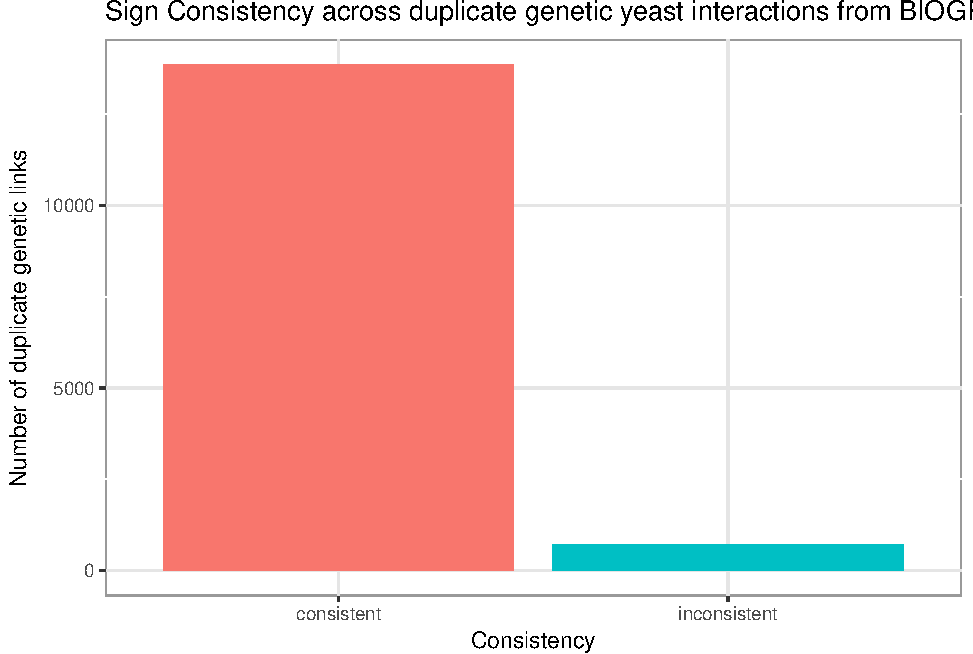
\includegraphics{yeast_GIN_files/figure-latex/unnamed-chunk-10-1.pdf}

\begin{Shaded}
\begin{Highlighting}[]
\NormalTok{count_consistency_GIN <-}\StringTok{ }\NormalTok{yeast_GIN_unique_dup2 %>%}
\StringTok{  }\KeywordTok{group_by}\NormalTok{(Consistency) %>%}
\StringTok{  }\KeywordTok{summarise} \NormalTok{(}\DataTypeTok{n =} \KeywordTok{n}\NormalTok{())}


\KeywordTok{kable}\NormalTok{(count_consistency_GIN, }\DataTypeTok{align =} \StringTok{'c'}\NormalTok{, }\DataTypeTok{caption =} \StringTok{"Sign consistency across duplicated genetic interactions in yeast GIN"}\NormalTok{)}
\end{Highlighting}
\end{Shaded}

\begin{longtable}[]{@{}cc@{}}
\caption{Sign consistency across duplicated genetic interactions in
yeast GIN}\tabularnewline
\toprule
Consistency & n\tabularnewline
\midrule
\endfirsthead
\toprule
Consistency & n\tabularnewline
\midrule
\endhead
consistent & 13844\tabularnewline
inconsistent & 718\tabularnewline
\bottomrule
\end{longtable}

Next we have to keep only the unique interactions and remove the
inconsistent interactions from the original dataset.

\begin{Shaded}
\begin{Highlighting}[]
\NormalTok{ddd <-}\StringTok{ }\KeywordTok{subset}\NormalTok{(yeast_GIN_unique_dup2,yeast_GIN_unique_dup2$Consistency==}\StringTok{"inconsistent"}\NormalTok{)}

\NormalTok{yeast_GIN$Consistency <-}\StringTok{ }\NormalTok{!(yeast_GIN$links %in%}\StringTok{ }\NormalTok{ddd$Dublicated_Interactions)}
\NormalTok{yeast_GIN$duplicate_not_first <-}\StringTok{ }\KeywordTok{duplicated}\NormalTok{(yeast_GIN$links)}
\NormalTok{yeast_GIN_final <-}\StringTok{ }\KeywordTok{subset}\NormalTok{(yeast_GIN, yeast_GIN$duplicate_not_first==}\OtherTok{FALSE}\NormalTok{)}
\NormalTok{yeast_GIN_final <-}\StringTok{ }\KeywordTok{subset}\NormalTok{(yeast_GIN_final, yeast_GIN_final$Consistency==}\OtherTok{TRUE}\NormalTok{)}


\KeywordTok{nrow}\NormalTok{(yeast_GIN_final)==}\KeywordTok{length}\NormalTok{(}\KeywordTok{unique}\NormalTok{(yeast_GIN_final$links)) }\CommentTok{# check unique links}
\end{Highlighting}
\end{Shaded}

\begin{verbatim}
## [1] TRUE
\end{verbatim}

\begin{Shaded}
\begin{Highlighting}[]
\KeywordTok{nrow}\NormalTok{(yeast_GIN_final)}
\end{Highlighting}
\end{Shaded}

\begin{verbatim}
## [1] 143448
\end{verbatim}

\begin{Shaded}
\begin{Highlighting}[]
\NormalTok{a <-}\StringTok{ }\KeywordTok{as.character}\NormalTok{(yeast_GIN_final$INTERACTOR_A)}
\NormalTok{b <-}\StringTok{ }\KeywordTok{as.character}\NormalTok{(yeast_GIN_final$INTERACTOR_B)}
\NormalTok{yeast_GIN_genes <-}\StringTok{ }\KeywordTok{as.data.frame}\NormalTok{(}\KeywordTok{unique}\NormalTok{(}\KeywordTok{c}\NormalTok{(a,b)))}
\NormalTok{yeast_GIN_genes <-}\StringTok{ }\NormalTok{yeast_GIN_final$INTERACTOR_B }\CommentTok{#as.factor(yeast_GIN_final$INTERACTOR_B))}

\KeywordTok{nrow}\NormalTok{(yeast_GIN_genes)}
\end{Highlighting}
\end{Shaded}

\begin{verbatim}
## NULL
\end{verbatim}

The removal of duplicates and the complete deletion of links with
duplicates and inconsistent signs leads to the final edgelist. The final
edgelist of yeast GIN consists of \textbf{143448} interactions and
\textbf{5433} genes.

\begin{Shaded}
\begin{Highlighting}[]
\NormalTok{count_weights_GIN <-}\StringTok{ }\NormalTok{yeast_GIN_final %>%}
\StringTok{  }\KeywordTok{group_by}\NormalTok{(weights) %>%}
\StringTok{  }\KeywordTok{summarise} \NormalTok{(}\DataTypeTok{n =} \KeywordTok{n}\NormalTok{())}


\KeywordTok{kable}\NormalTok{(count_weights_GIN, }\DataTypeTok{align =} \StringTok{'c'}\NormalTok{, }\DataTypeTok{caption =} \StringTok{"Weight frequences of the yeast GIN"}\NormalTok{)}
\end{Highlighting}
\end{Shaded}

\begin{longtable}[]{@{}cc@{}}
\caption{Weight frequences of the yeast GIN}\tabularnewline
\toprule
weights & n\tabularnewline
\midrule
\endfirsthead
\toprule
weights & n\tabularnewline
\midrule
\endhead
-1 & 114864\tabularnewline
1 & 28584\tabularnewline
\bottomrule
\end{longtable}

\subsection{Loops}\label{loops}

Next, we need to examine if there are any loops in the network. Which
means that we have to look for interactions that have the same gene in
edge list.

\begin{Shaded}
\begin{Highlighting}[]
\NormalTok{loop_finder <-}\StringTok{ }\NormalTok{function(x)\{}
  \NormalTok{d<-}\StringTok{ }\KeywordTok{c}\NormalTok{()}
  \NormalTok{for(i in }\DecValTok{1}\NormalTok{:}\KeywordTok{nrow}\NormalTok{(x))\{}
   
    \NormalTok{if(}\KeywordTok{as.character}\NormalTok{(x[i,}\DecValTok{1}\NormalTok{])==}\KeywordTok{as.character}\NormalTok{(x[i,}\DecValTok{2}\NormalTok{]))\{}
      \NormalTok{d <-}\StringTok{ }\KeywordTok{c}\NormalTok{(d,}\KeywordTok{as.character}\NormalTok{(x[i,}\DecValTok{1}\NormalTok{]))}
    \NormalTok{\}else\{\}}
  \NormalTok{\}}
    \NormalTok{d <-}\KeywordTok{as.data.frame}\NormalTok{(d)}
    \KeywordTok{colnames}\NormalTok{(d)[}\DecValTok{1}\NormalTok{]<-}\StringTok{"genes_loop"}  
    \NormalTok{d}
  \NormalTok{\}}
\NormalTok{loops <-}\StringTok{ }\KeywordTok{loop_finder}\NormalTok{(yeast_GIN_final) }
\KeywordTok{nrow}\NormalTok{(loops)}
\end{Highlighting}
\end{Shaded}

\begin{verbatim}
## [1] 8
\end{verbatim}

There are 8 loops in the yeast GIN. What do they mean? Do they have
biological meaning?

\section{Network analysis}\label{network-analysis}

Import the network in igraph. We choose to delete the loops (8).

\begin{Shaded}
\begin{Highlighting}[]
\KeywordTok{library}\NormalTok{(igraph)}

\NormalTok{yeast_GIN_Net <-}\StringTok{ }\KeywordTok{as.data.frame}\NormalTok{(yeast_GIN_final[,-}\KeywordTok{c}\NormalTok{(}\DecValTok{3}\NormalTok{:}\DecValTok{11}\NormalTok{,}\DecValTok{13}\NormalTok{:}\DecValTok{16}\NormalTok{)])}
\NormalTok{g_yeast_GIN <-}\StringTok{ }\KeywordTok{graph_from_data_frame}\NormalTok{(yeast_GIN_Net,}\DataTypeTok{directed =} \NormalTok{T)}
\KeywordTok{summary}\NormalTok{(g_yeast_GIN)}
\end{Highlighting}
\end{Shaded}

\begin{verbatim}
## IGRAPH DN-- 5433 143448 -- 
## + attr: name (v/c), weights (e/n)
\end{verbatim}

\begin{Shaded}
\begin{Highlighting}[]
\KeywordTok{is.simple}\NormalTok{(g_yeast_GIN)}
\end{Highlighting}
\end{Shaded}

\begin{verbatim}
## [1] FALSE
\end{verbatim}

\begin{Shaded}
\begin{Highlighting}[]
\CommentTok{#It has multiple links? }
\KeywordTok{E}\NormalTok{(g_yeast_GIN)$multiple <-}\StringTok{ }\KeywordTok{which_multiple}\NormalTok{(g_yeast_GIN)}
\KeywordTok{summary}\NormalTok{(}\KeywordTok{E}\NormalTok{(g_yeast_GIN)$multiple) }\CommentTok{# all FALSE}
\end{Highlighting}
\end{Shaded}

\begin{verbatim}
##    Mode   FALSE    NA's 
## logical  143448       0
\end{verbatim}

\begin{Shaded}
\begin{Highlighting}[]
\CommentTok{# It has loops?   }
\KeywordTok{E}\NormalTok{(g_yeast_GIN)$loop <-}\StringTok{ }\KeywordTok{which_loop}\NormalTok{(g_yeast_GIN)}
\KeywordTok{summary}\NormalTok{(}\KeywordTok{E}\NormalTok{(g_yeast_GIN)$loop) }\CommentTok{# 8 TRUE loops}
\end{Highlighting}
\end{Shaded}

\begin{verbatim}
##    Mode   FALSE    TRUE    NA's 
## logical  143440       8       0
\end{verbatim}

\begin{Shaded}
\begin{Highlighting}[]
\CommentTok{#Remove loops}
\NormalTok{g_yeast_GIN <-}\StringTok{ }\NormalTok{igraph::}\KeywordTok{simplify}\NormalTok{(g_yeast_GIN)}
\CommentTok{# Assign attributes}
\NormalTok{yeast_GIN_Net$sign_color <-}\StringTok{ }\KeywordTok{with}\NormalTok{(yeast_GIN_Net, }\KeywordTok{ifelse}\NormalTok{(weights<}\DecValTok{0}\NormalTok{, }\KeywordTok{paste0}\NormalTok{(}\StringTok{"red"}\NormalTok{), }\KeywordTok{paste0}\NormalTok{(}\StringTok{"blue"}\NormalTok{)))}
\KeywordTok{E}\NormalTok{(g_yeast_GIN)$weights <-}\StringTok{ }\NormalTok{yeast_GIN_Net$weights}
\KeywordTok{E}\NormalTok{(g_yeast_GIN)$sign_color <-}\StringTok{ }\NormalTok{yeast_GIN_Net$sign_color}
\KeywordTok{is.simple}\NormalTok{(g_yeast_GIN)}
\end{Highlighting}
\end{Shaded}

\begin{verbatim}
## [1] TRUE
\end{verbatim}

\begin{Shaded}
\begin{Highlighting}[]
\KeywordTok{summary}\NormalTok{(g_yeast_GIN)}
\end{Highlighting}
\end{Shaded}

\begin{verbatim}
## IGRAPH DN-- 5433 143440 -- 
## + attr: name (v/c), weights (e/n), sign_color (e/c)
\end{verbatim}

Create the adjacency matrix.

\begin{Shaded}
\begin{Highlighting}[]
\NormalTok{adjacency_weight_yeast_GIN <-}\StringTok{ }\KeywordTok{as_adjacency_matrix}\NormalTok{(g_yeast_GIN, }\DataTypeTok{attr =} \StringTok{"weights"}\NormalTok{,}\DataTypeTok{names =} \NormalTok{T)}
\NormalTok{adjacency_weight_yeast_GIN <-}\StringTok{ }\KeywordTok{as.data.frame}\NormalTok{(}\KeywordTok{as.matrix}\NormalTok{(adjacency_weight_yeast_GIN))}
\KeywordTok{sum}\NormalTok{(}\KeywordTok{sapply}\NormalTok{(adjacency_weight_yeast_GIN,is.character)) }\CommentTok{# if 0 then there are no characters inside dataframe!}
\end{Highlighting}
\end{Shaded}

\begin{verbatim}
## [1] 0
\end{verbatim}

\begin{Shaded}
\begin{Highlighting}[]
\CommentTok{#write.table(adjacency_weight_yeast_GIN,file = "adjacency_matrix_yeast_GIN.txt",sep = "\textbackslash{}t",row.names = T,col.names = T) # the file of the adjacency matrix.}
\end{Highlighting}
\end{Shaded}

To make further calculations we isolate the giant component.

\begin{Shaded}
\begin{Highlighting}[]
\NormalTok{igraph::}\KeywordTok{is.connected}\NormalTok{(g_yeast_GIN)}
\end{Highlighting}
\end{Shaded}

\begin{verbatim}
## [1] FALSE
\end{verbatim}

\begin{Shaded}
\begin{Highlighting}[]
\NormalTok{decg<-}\KeywordTok{decompose.graph}\NormalTok{(g_yeast_GIN, }\DataTypeTok{min.vertices =} \DecValTok{10}\NormalTok{) }\CommentTok{#upografima tis megalis sinistosas }
\NormalTok{gcomp_GIN<-decg[[}\DecValTok{1}\NormalTok{]]}
\NormalTok{igraph::}\KeywordTok{is.connected}\NormalTok{(gcomp_GIN)}
\end{Highlighting}
\end{Shaded}

\begin{verbatim}
## [1] TRUE
\end{verbatim}

\begin{Shaded}
\begin{Highlighting}[]
\KeywordTok{summary}\NormalTok{(gcomp_GIN)}
\end{Highlighting}
\end{Shaded}

\begin{verbatim}
## IGRAPH DN-- 5422 143431 -- 
## + attr: name (v/c), weights (e/n), sign_color (e/c)
\end{verbatim}

Only 11 genes and 9 links weren't connected with the giant component.

\subsection{Degree distribution}\label{degree-distribution}

One of the first things to examine is the degree distribution of the
graph.

\begin{Shaded}
\begin{Highlighting}[]
\CommentTok{# Degree distribution of the graph}

\NormalTok{de <-}\StringTok{ }\NormalTok{igraph::}\KeywordTok{degree}\NormalTok{(gcomp_GIN)}
\NormalTok{de <-}\StringTok{ }\KeywordTok{as.data.frame}\NormalTok{(de)}
\NormalTok{de$node <-}\StringTok{ }\KeywordTok{c}\NormalTok{(}\KeywordTok{seq}\NormalTok{(}\DecValTok{1}\NormalTok{:}\KeywordTok{length}\NormalTok{(de$de)))}
\NormalTok{dd<-}\KeywordTok{aggregate}\NormalTok{(}\KeywordTok{rep.int}\NormalTok{(}\DecValTok{1}\NormalTok{, }\KeywordTok{length}\NormalTok{(de$node))~de$de, }\DataTypeTok{FUN=}\NormalTok{sum)}
\KeywordTok{names}\NormalTok{(dd)<-}\KeywordTok{c}\NormalTok{(}\StringTok{"val"}\NormalTok{,}\StringTok{"freq"}\NormalTok{)}

\KeywordTok{ggplot}\NormalTok{()+}
\StringTok{  }\KeywordTok{geom_point}\NormalTok{(}\DataTypeTok{data =} \NormalTok{dd, }\KeywordTok{aes}\NormalTok{(}\DataTypeTok{x =} \NormalTok{val,}\DataTypeTok{y =} \NormalTok{freq ),}\DataTypeTok{color=}\StringTok{"red"}\NormalTok{)+}
\StringTok{  }\KeywordTok{scale_y_log10}\NormalTok{()+}
\StringTok{  }\KeywordTok{scale_x_log10}\NormalTok{()+}
\StringTok{  }\KeywordTok{ggtitle}\NormalTok{(}\StringTok{"Degree Distribution of Yeast Genetic Interactions Network"}\NormalTok{)+}
\StringTok{  }\KeywordTok{labs}\NormalTok{(}\DataTypeTok{x=}\StringTok{"Log10(node degree)"}\NormalTok{, }\DataTypeTok{y=}\StringTok{"log10(frequency of degree)"}\NormalTok{)+}
\StringTok{  }\KeywordTok{theme_bw}\NormalTok{()}
\end{Highlighting}
\end{Shaded}

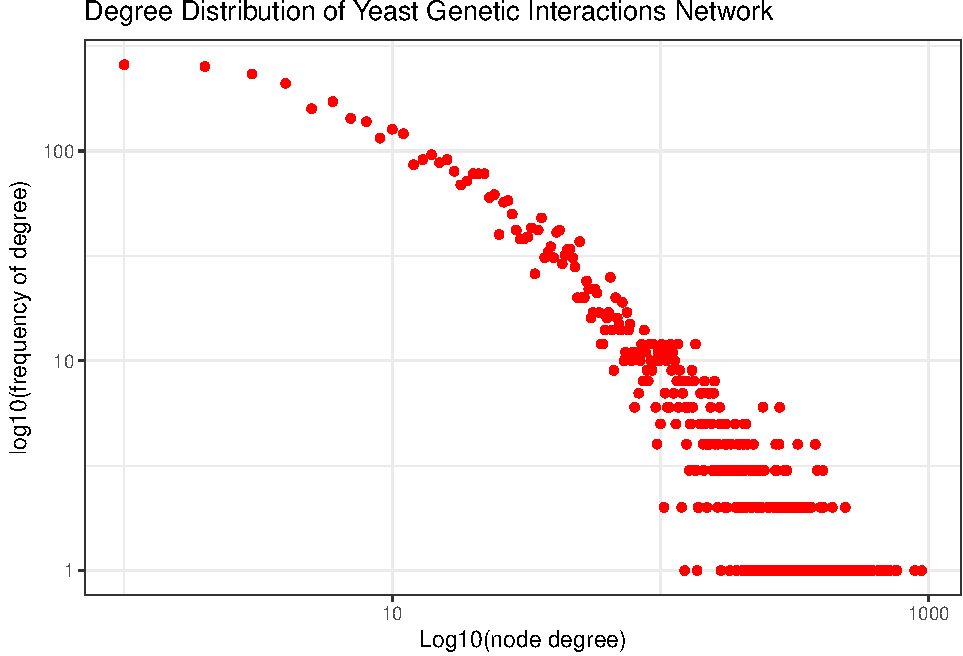
\includegraphics{yeast_GIN_files/figure-latex/unnamed-chunk-17-1.pdf}

Plot of the network.

\begin{Shaded}
\begin{Highlighting}[]
\NormalTok{layg <-}\StringTok{ }\KeywordTok{layout_nicely}\NormalTok{(gcomp_GIN)}
\KeywordTok{V}\NormalTok{(gcomp_GIN)$coord1 <-layg[ ,}\DecValTok{1}\NormalTok{]     ## network plots}
\KeywordTok{V}\NormalTok{(gcomp_GIN)$coord2 <-layg[ ,}\DecValTok{2}\NormalTok{]}

\KeywordTok{plot}\NormalTok{(gcomp_GIN, }
     \DataTypeTok{layout=}\NormalTok{layg,}
     \DataTypeTok{vertex.shape=}\StringTok{"circle"}\NormalTok{, }
     \DataTypeTok{vertex.size=}\FloatTok{0.0095}\NormalTok{, }
     \DataTypeTok{vertex.color=}\StringTok{"green"}\NormalTok{,  }
     \DataTypeTok{vertex.frame.color=}\StringTok{"green"}\NormalTok{,}
     \DataTypeTok{vertex.label=}\OtherTok{NA}\NormalTok{, }
     \CommentTok{#vertex.label.cex = vcount(g)*0.00004,}
     \CommentTok{#vertex.label.color ="black", }
     \DataTypeTok{edge.color=}\KeywordTok{E}\NormalTok{(gcomp_GIN)$sign_color,}
     \DataTypeTok{edge.width=}\FloatTok{0.03}\NormalTok{, }
     \DataTypeTok{edge.arrow.size =} \FloatTok{0.00001}\NormalTok{,}
     \DataTypeTok{edge.arrow.width =} \FloatTok{0.0000005}\NormalTok{,}
     \CommentTok{#edge.label=round(x = E(g)$weight,digits = 3), }
     \CommentTok{#edge.label.cex = 0.3,}
     \CommentTok{#edge.label.color = E(g)$color,}
     \DataTypeTok{margin =} \DecValTok{0}\NormalTok{,}
     \DataTypeTok{main =} \StringTok{""}\NormalTok{,}
     \DataTypeTok{sub =} \StringTok{""}\NormalTok{)}
\KeywordTok{title}\NormalTok{(}\DataTypeTok{main =} \KeywordTok{paste}\NormalTok{(}\StringTok{"yeast GIN network "}\NormalTok{), }\DataTypeTok{cex.main=} \FloatTok{1.5}\NormalTok{, }\DataTypeTok{cex.sub =} \FloatTok{1.2}\NormalTok{,}\DataTypeTok{outer =} \NormalTok{F)}
\end{Highlighting}
\end{Shaded}

\includegraphics{yeast_GIN_files/figure-latex/unnamed-chunk-18-1.pdf}

\begin{Shaded}
\begin{Highlighting}[]
\CommentTok{#sss <- induced_subgraph(gcomp_GIN, v = nei[[1]])}

\CommentTok{#plot(sss,edge.color=E(gcomp_GIN)$sign_color)}

\CommentTok{#nei <- neighborhood(gcomp_GIN,order = 1,nodes = "YOL001W")}

\NormalTok{yeast_GIN_final$AD <-}\StringTok{ }\KeywordTok{paste0}\NormalTok{(yeast_GIN_final[,}\DecValTok{1}\NormalTok{],}\StringTok{","}\NormalTok{,yeast_GIN_final[,}\DecValTok{12}\NormalTok{])}
\NormalTok{yeast_GIN_final$BD <-}\StringTok{ }\KeywordTok{paste0}\NormalTok{(yeast_GIN_final[,}\DecValTok{2}\NormalTok{],}\StringTok{","}\NormalTok{,yeast_GIN_final[,}\DecValTok{12}\NormalTok{])}

\NormalTok{AD_freq <-}\StringTok{ }\KeywordTok{table}\NormalTok{(yeast_GIN_final$AD)}
\NormalTok{AD_freq <-}\StringTok{ }\KeywordTok{as.data.frame}\NormalTok{(AD_freq)}
\NormalTok{BD_freq <-}\StringTok{ }\KeywordTok{table}\NormalTok{(yeast_GIN_final$BD)}


\NormalTok{AD_freq_a <-}\StringTok{ }\KeywordTok{strsplit}\NormalTok{(}\KeywordTok{as.character}\NormalTok{(AD_freq$Var1),}\DataTypeTok{split =} \StringTok{","}\NormalTok{)}
\NormalTok{AD_freq_a <-}\StringTok{ }\KeywordTok{as.data.frame}\NormalTok{(AD_freq_a)}
\NormalTok{AD_freq_a <-}\StringTok{ }\KeywordTok{t}\NormalTok{(AD_freq_a)}

\NormalTok{AD_freq$gene <-}\StringTok{ }\NormalTok{AD_freq_a[,}\DecValTok{1}\NormalTok{]}
\NormalTok{AD_freq$weight <-}\StringTok{ }\NormalTok{AD_freq_a[,}\DecValTok{2}\NormalTok{]}

\NormalTok{AD_freq_a_1 <-}\StringTok{ }\NormalTok{AD_freq[}\KeywordTok{order}\NormalTok{(AD_freq$weight,AD_freq$Freq,}\DataTypeTok{decreasing =} \NormalTok{T),]}
\NormalTok{AD_freq_a_neg <-}\StringTok{ }\KeywordTok{subset}\NormalTok{(}\DataTypeTok{x =} \NormalTok{AD_freq_a_1,AD_freq_a_1$weight==-}\DecValTok{1}\NormalTok{)}
\CommentTok{#AD_freq_a_1 <- AD_freq[order(AD_freq$Freq,decreasing = T),]}
\end{Highlighting}
\end{Shaded}


\end{document}
